\documentclass[12pt]{article}

\usepackage[english]{babel}
\usepackage{graphicx}
\usepackage{setspace}
\usepackage{parskip}
\usepackage{indentfirst}
\usepackage{courier}
\usepackage{hyperref}
\usepackage{enumerate}
\usepackage{vhistory}

\pagestyle{empty}
\setcounter{secnumdepth}{2}

\topmargin=0cm
\oddsidemargin=0cm
\textheight=22.0cm
\textwidth=16cm
\parindent=1cm
\parskip=0.15cm
\topskip=0truecm
\raggedbottom
\abovedisplayskip=3mm
\belowdisplayskip=3mm
\abovedisplayshortskip=0mm
\belowdisplayshortskip=2mm
\normalbaselineskip=12pt
\normalbaselines

\begin{document}

%%%%%%%%%%%%%%%%%%%%%%%%%%%%%%%%%%%%%%%%%%%%%%%%%%%%%%%%%%%%%%
%                        First page                         
%%%%%%%%%%%%%%%%%%%%%%%%%%%%%%%%%%%%%%%%%%%%%%%%%%%%%%%%%%%%%%


\vspace*{0.5in}
\centerline{\bf\Large Deliverable 3}
\vspace*{0.2in}
\centerline{\bf\Large Project Testing and Delivery Document}

\vspace*{1.7in}
\centerline{\bf\Large C-Lab}
\vspace*{0.2in}
\centerline{
\begin{tabular}{c c}
      Ashwath George & 9733469\\
      Nicholas Gignac & 9128964\\
      Robert Jakubowicz & 6045707\\
      Caroline Labbe & 6320945\\
      Brian Lam & 1696785\\\\
\end{tabular}}

\vspace*{1.2in}
\centerline{\bf\Large For the course:}
\centerline{\bf\Large COMP354}
\centerline{\bf\Large Introduction to Software Engineering}

\vspace*{0.8in}
\centerline{Presented to:}
\centerline{Sutharsan Sivagnanam}
\centerline{August 14, 2013}

\clearpage

% Revision history
\begin{versionhistory}
  \vhEntry{0.0}{07/08/13}{Caroline}{Added Latex template}
  \vhEntry{0.1}{07/08/13}{Nicholas}{Added introduction}
  \vhEntry{0.2}{08/08/13}{Brian}   {Added test coverage}
  \vhEntry{0.3}{09/08/13}{Robert}  {Added unit test cases}
  \vhEntry{0.4}{10/08/13}{Ashwath} {Added requirements test scenarios}
  \vhEntry{0.5}{10/08/13}{Nicholas}{Added installation and user manual}
  \vhEntry{0.6}{11/08/13}{Nicholas}{Added stress testing}
  \vhEntry{0.7}{12/08/13}{Nicholas}{Added final cost estimate}
  \vhEntry{0.8}{12/08/13}{Caroline}{Fix latex formatting}
  \vhEntry{0.9}{12/08/13}{Caroline}{Insert figures at the right places}
  \vhEntry{1.0}{12/08/13}{Caroline}{Assemble all sections to complete document}
  \vhEntry{1.1}{13/08/13}{Caroline}{Fix some typos after review}
\end{versionhistory}
\clearpage

\setcounter{secnumdepth}{3}
\tableofcontents
\clearpage
\listoffigures
\listoftables

\clearpage

\pagestyle{plain}
\doublespacing


%%%%%%%%%%%%%%%%%%%%%%%%%%%%%%%%%%%%%%%%%%%%%%%%%%%%%%%%%%%%%%
%                       Introduction                        
%%%%%%%%%%%%%%%%%%%%%%%%%%%%%%%%%%%%%%%%%%%%%%%%%%%%%%%%%%%%%%


\section{Introduction}
\par
The C-Ker Vessel Monitoring System, from C-Lab, has been completed and the final iteration has been demoed successfully. This document will provide a detailed analysis of the various tests performed on the system prior to its submission, as well as the corresponding results subsequently obtained. An installation and user manual will also be included, as well as the final revision of the Cost Estimation of the system’s development.




%%%%%%%%%%%%%%%%%%%%%%%%%%%%%%%%%%%%%%%%%%%%%%%%%%%%%%%%%%%%%%
%                       Testing Report                     
%%%%%%%%%%%%%%%%%%%%%%%%%%%%%%%%%%%%%%%%%%%%%%%%%%%%%%%%%%%%%%



\section{Testing Report}

\subsection{Test Coverage}
\subsubsection{Tested Items}
The tested items can be categorized into requirements and units.\\


\leftline{\textsc{Tested Requirements}}
\vspace*{0.2in}
All application features are tested thoroughly. However, mandatory functionalities listed in the requirement specification document are treated with a higher priority.

\begin{itemize}
\item Listing Vessels in a Table\par
This is a core feature which allows users to view vessel information in a list.
\item Displaying Vessels on a Radar\par
This is a core feature which allows users to visualize vessels graphically.
\item Filtering Vessels by Type\par
This is a core feature which allows users to view only specific vessel types.
\item Sorting Vessels by Attribute\par
This is a core feature which allows users to organize vessel information by data.
\item Loading Vessel Scenario Files\par
This is a core functionality which allows the application to load simulation properties.
\item Simulating Vessel Movement\par
This is a core functionality which allows the application to have moving vessels.
\item Triggering Risk Alarms\par
This is a core functionality which allows the application to display alarm alerts in both the table and the radar when vessels get too close to each other.
\item Login Authentication\par
This is a core functionality which allows users to login as either an administrator or an operator; only administrators can filter and sort vessels.
\item Maximum of 100 Vessels in Simulation\par
This is a mandatory non-functional requirement which allows the simulation to handle up to one hundred vessels at the same time.
\item Shortest Time Step of 0.5 Seconds in Simulation\par
This is a mandatory non-functional requirement which allows the simulation to update at a time step from 0.5 seconds and up.
\end{itemize}

\clearpage

\leftline{\textsc{Tested Units}}
The tested units include the ScenarioParser, the Authenticator, the Vessel, the VesselPresenter, and the LoginPresenter classes.
\begin{itemize}
\item ScenarioParser\par
This class takes care of parsing and loading scenario files. It is important to test because the simulation entirely depends on the success of the file data being loaded correctly. In addition to reading the file accurately, it should also reject files that are not properly formatted.
\item Authenticator\par
This class takes care of authenticator user login attempts. It is important to test in order to ensure that user privileges are enforced correctly. Only a correct combination of username and password may access the application's main window.  
\item Vessel\par
This class encapsulates vessel data and methods. It is important to test that the distance between two vessels is calculated correctly, so that alarms can be generated properly. It is also important test that the vessel positions are updated correctly, so that the simulation can run properly.
\item VesselPresenter\par
This class presents the vessel information to be displayed by the interface; it also takes care of sorting and filtering vessels. It is important to test because sorting and filtering are core features which are used fairly frequently by the user. The filtering function should remove unwanted vessel types from the list of vessels displayed, while the sorting function should order the list of vessels displayed by a specified attribute.
\item LoginPresenter\par
This class presents authentication information to the login screen. It is important to test in order to ensure correct functionality of the login screen. The correct user type should be identified properly when given a specific user.
\end{itemize}


\subsubsection{Untested Items of Interest}
The vessel data from the scenario files are not tested for realism or plausibility; it is accepted as long as the formatting is correct. In other words, it is entirely possible that certain vessel types go at very unrealistic speeds, such as a human going 340 meters per second. In order to reject unrealistic scenarios, further research on vessel types must be performed. It then becomes a simple matter of testing maximum and minimum value constraints. In our case, it is up to the user to provide a scenario that makes sense.

\subsection{Test Cases}

\subsubsection{Unit Testing}

\centerline{\textsc{ScenarioParser class}}
\vspace*{0.2in}

The ScenarioParser class is tested using white box testing since it has been developed by us. The tests are in the class ParserTest.cs which is run by NUnit. This class takes care parsing scenario files and extracting information that goes into the vessels list or details about the simulation.

\clearpage

{\bfseries ParseText (string text)} \newline
{\bfseries Condition:} Text is empty \newline
{\bfseries Description:} This test inputs an empty string and checks that no vessel is returned.\\

\texttt{public void ParseText\_EmptyText\_ReturnsEmptyList()}\\
\texttt{\{}\par
\texttt{string text = "\textbackslash n";}\par
\texttt{List<Vessel> actual = ScenarioParser.ParseText(text);}\par
\texttt{List<Vessel> expected = new List<Vessel>();}\par	 
\texttt{Assert.AreEqual(expected.Count, actual.Count);}\\
\texttt{\}}\\


{\bfseries ParseText (string text)} \newline
{\bfseries Condition:} Text is a valid vessel line \newline
{\bfseries Description:} This test inputs a string with each field of a vessel and checks that each field on the returned vessel matches.\\

\texttt{public void ParseText\_ValidLine\_ReturnsListWithOneVesselObject()}\\
\texttt{\{}\par
\texttt{string text = "NEWT 001 1 4990 0 0.1 0.1 10\textbackslash n";}\par
\texttt{List<Vessel> actual = ScenarioParser.ParseText(text);}\par
\texttt{List<Vessel> expected = new List<Vessel>();}\par
\texttt{expected.Add(new Vessel(new string[] { "NEWT", "1", "1", "4990", "0", "0.1", "0.1", "10" }));}\par
\vspace{5 mm}
\texttt{Assert.AreEqual(expected.Count, actual.Count);}\par
\vspace{5 mm}
\texttt{for (int i = 0; i != expected.Count; i++)}\par
\texttt{\{}\par
\texttt{Assert.IsTrue(new VesselComparer().Equals(expected[i], actual[i]));}\par
\texttt{\}}\\
\texttt{\}}\\



{\bfseries ParseText (string text)} \newline
{\bfseries Condition:} Text line is missing NEWT \newline
{\bfseries Description:} This test inputs a string with a missing NEWT at the beginning and checks that no vessel is returned.\\

\texttt{public void ParseText\_InvalidLineMissing\_ReturnsZero()}\\
\texttt{\{}\par
\texttt{string text = "001         	 1   		 4990      			 0   			 0.1   		   	 	0.1 		  10\textbackslash n";}\par
\texttt{List<Vessel> actual   = ScenarioParser.ParseText(text);}\par
\texttt{int expected = 0;}\par     
\texttt{Assert.AreEqual(expected, actual.Count);}\\
\texttt{\}}\\



{\bfseries ParseText (string text)} \newline
{\bfseries Condition:} Text contains an invalid value \newline
{\bfseries Description:} This test inputs a string where an numerical value is expected but a letter is given. It then checks that a FormatException is thrown.\\
\vspace*{0.2in}
\texttt{public void ParseText\_InvalidLineValue\_ThrowsFormatException()}\\
\texttt{\{}\par
\texttt{Assert.Throws<System.FormatException>(}\par
\texttt{delegate}\par
\texttt{\{}\par
\texttt{string text = "NEWT 001              1   		 4990      			 a   			 0.1   		   	 	0.1 		  10\textbackslash n";}\par 
\texttt{ScenarioParser.ParseText(text);}\par
\texttt{\}}\par
\texttt{);}\\
\texttt{\}}\\



{\bfseries ParseText (string text)} \newline
{\bfseries Condition:} Text contains an undefined keyword \newline
{\bfseries Description:} This test inputs a string with the keyword NOTEXISTING and then checks that no vessel is returned.\\

\texttt{public void ParseText\_InvalidLineKeyword\_ReturnsZero()}\\
\texttt{\{}\par
\texttt{string text = "NOTEXISTING 001          1   	 4990      			 0   			 0.1   		   	 	0.1 		  10\textbackslash n";}\par
\texttt{List<Vessel> actual = ScenarioParser.ParseText(text);}\par
\texttt{int expected = 0;}\par     
\texttt{Assert.AreEqual(expected, actual.Count);}\\
\texttt{\}}



{\bfseries ParseText (string text)} \newline
{\bfseries Condition:} Text contains details about the simulation: starttime, timestep, time and range and the value are integers. \newline
{\bfseries Description:} This test inputs a string with integer values for the simulation details. It then checks that the ScenarioParser.Simulator contains the correct values.\\

\texttt{public void ParseText\_ValidSimulationIntegerDetails\_ReturnsFilledScenarionParser\_Simulator()}\\
\texttt{\{}\par
\texttt{string text = "STARTTIME 0\textbackslash n" + "TIMESTEP 1\textbackslash n" + "TIME 500\textbackslash n" + "RANGE 500\textbackslash n" ;
}\par
\texttt{ScenarioParser.ParseText(text);}\par
\texttt{float expectedStartTime = 0f;}\par     
\texttt{float expectedTimeStep = 1f;}\par
\texttt{float expectedTime = 500f;}\par
\texttt{int expectedRange = 500;}\par
\texttt{Assert.AreEqual(expectedStartTime, ScenarioParser.Simulator.StartTime, float.Epsilon);}\par
\texttt{Assert.AreEqual(expectedTimeStep, ScenarioParser.Simulator.TimeStep, float.Epsilon);}\par
\texttt{Assert.AreEqual(expectedTime, ScenarioParser.Simulator.Time, float.Epsilon);}\par
\texttt{Assert.AreEqual(expectedRange, ScenarioParser.Simulator.Range);}\\
\texttt{\}}

\clearpage

{\bfseries ParseText (string text)} \newline
{\bfseries Condition:} Text contains details about the simulation: starttime, timestep, time and range and the value are floats.\newline
{\bfseries Description:} This test inputs a string with float values for the simulation details. It then checks that the ScenarioParser.Simulator contains the correct values.\\

\texttt{public void ParseText\_ValidSimulationFloatDetails\_ReturnsFilledScenarionParser\_Simulator()}\\
\texttt{\{}\par
\texttt{string text = string text = "STARTTIME 0.3\textbackslash n" + "TIMESTEP 1.1\textbackslash n" + "TIME 500.5\textbackslash n" + "RANGE 500\textbackslash n";}\par
\texttt{ScenarioParser.ParseText(text);}\par
\texttt{float expectedStartTime = 0.3f;}\par     
\texttt{float expectedTimeStep = 1.1f;}\par
\texttt{float expectedTime = 500.5f;}\par
\texttt{int expectedRange = 500;}\par
\texttt{Assert.AreEqual(expectedStartTime, ScenarioParser.Simulator.StartTime, float.Epsilon);}\par
\texttt{Assert.AreEqual(expectedTimeStep, ScenarioParser.Simulator.TimeStep, float.Epsilon);}\par
\texttt{Assert.AreEqual(expectedTime, ScenarioParser.Simulator.Time, float.Epsilon);}\\
\texttt{\}}

\clearpage

{\bfseries ParseText (string text)} \newline
{\bfseries Condition:} Text contains details about the simulation that are invalid. \newline
{\bfseries Description:} This test inputs a string of integer values for the simulation details where some values are letters instead of numeric. It then checks that a FormatException is thrown.\\

\texttt{public void ParseText\_InvalidSimulationDetails\_ThrowsFormatException()}\\
\texttt{\{}\par
\texttt{string text = "STARTTIME 0\textbackslash n" + "TIMESTEP A\textbackslash n" + "TIME B\textbackslash n" + "RANGE 500\textbackslash n";}\par
\texttt{Assert.Throws<System.FormatException>(}\par
\texttt{delegate}\par     
\texttt{\{}\par
\texttt{ScenarioParser.ParseText(text);}\par
\texttt{\}}\par
\texttt{);}\\
\texttt{\}}\par

\clearpage

{\bfseries Results} \newline
Figure~\ref{fig:ScenarioParser class} shows the results as run from NUnit. It shows all the tests passing.
\begin{figure}[h!]
    \centering
    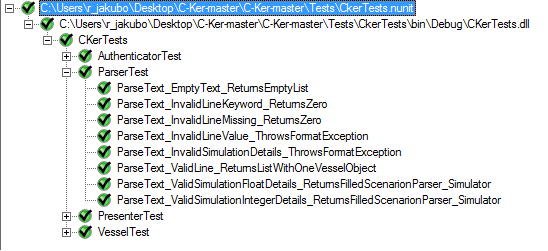
\includegraphics[scale=0.8]{ScenarioParser_class}
    \caption{ScenarioParser class}
    \label{fig:ScenarioParser class}
\end{figure}



\centerline{\textsc{Authenticator class}}
\vspace*{0.2in}
The Authenticator class is tested using white box testing since it has been developed by us. The tests are in the class AuthenticatorTest.cs which is run by NUnit. This class takes care of correctly identifying valid user and rejecting invalid ones. Hence, different username and password combinations must be thoroughly tested.\\


{\bfseries FindUser(string username)}\\
{\bfseries Condition:} Invalid username\\
{\bfseries Description:} This test inputs an invalid username and check that no user is returned.\\
\clearpage
\texttt{public void FindUser\_InvalidUsername\_ReturnsNull()}\\
\texttt{\{}\par
\texttt{string username = "InvalidUsername";}\par
\texttt{User actual = Authenticator.FindUser(username);}\par
\texttt{Assert.IsNull(actual);}\\
\texttt{\}}\\



{\bfseries FindUser(string username)}\\
{\bfseries Condition:} Valid username\\
{\bfseries Description:} This test inputs a valid username and check that a valid user object is returned.\\
\texttt{public void FindUser\_ValidUsername\_ReturnsInstanciatedUserObject()}\\
\texttt{\{}\par
\texttt{string username = "admin";}\par
\texttt{User expected = new User();}\par
\texttt{expected.Name = username;}\par  	 
\texttt{User actual = Authenticator.FindUser(username);}\par
\texttt{Assert.AreEqual(expected.ToString(), actual.ToString());}\\
\texttt{\}}\\

{\bfseries FindUser(string username, string password)}\\
{\bfseries Condition:} Invalid username and password\\
{\bfseries Description:} This test inputs an invalid username and password and check that no user is returned.\\
\texttt{public void FindUser\_InvalidUsernameAndPassword\_ReturnsNull()}\\
\texttt{\{}\par
\texttt{string username = "InvalidUsername";}\par
\texttt{string password = "InvalidPassword";}\par
\texttt{User actual = Authenticator.FindUser(username, password);}\par
\texttt{Assert.IsNull(actual);}\\
\texttt{\}}\\

{\bfseries FindUser(string username, string password)}\\
{\bfseries Condition:} Valid username and password\\
{\bfseries Description:} This test inputs a valid username and password check that a valid user object is returned.\\
\texttt{public void FindUser\_ValidUsernameAndPassword\_ReturnsInstanciatedUserObject()}\\
\texttt{\{}\par
\texttt{string username = "admin";}\par
\texttt{string password = "fullaccess";}\par
\texttt{User expected = new User();}\par
\texttt{expected.Name = username;}\par
\texttt{expected.Password = password;}\par
\texttt{User actual = Authenticator.FindUser(username, password);}\par
\texttt{Assert.AreEqual(expected.ToString(), actual.ToString());}\\
\texttt{\}}
    
    \clearpage
    
{\bfseries Logout()}\\
{\bfseries Condition:} A user is logged in\\
{\bfseries Description:} This tests logs in a valid user and check that no user is logged in after logout() is called.\\

\texttt{public void Logout\_AUserLoggedIn\_ReturnsNull()}\\
\texttt{\{}\par
\texttt{Authenticator.Login("admin", "fullaccess");}\par
\texttt{Authenticator.Logout();}\par
\texttt{Assert.IsNull(Authenticator.CurrentUser);}\\
\texttt{\}}\\

{\bfseries Login(string username, string password)}\\
{\bfseries Condition:} Invalid username and password\\
{\bfseries Description:} This tests inputs an invalid username and password and tries to login that user. Since they are invalid, it checks that no user is logged in.\\

\texttt{public void Login\_InvalidUser\_ReturnsCurrentUserNull()}\\
\texttt{\{}\par
\texttt{Authenticator.Login("adminfake", "fullaccessfake");}\par
\texttt{Assert.IsNull(Authenticator.CurrentUser);}\\	 
\texttt{\}}

\clearpage

{\bfseries Login(string username, string password)}\\
{\bfseries Condition:} Valid username and password\\
{\bfseries Description:} This tests inputs a valid username and password and tries to login that user. Since they are valid, it checks that a valid user is logged in.\\

\texttt{public void Login\_ValidUser\_ReturnsMatchingUsernameAndPassword()}\\
\texttt{\{}\par       	 
\texttt{Authenticator.Login("admin", "fullaccess");}\par  	 
\texttt{string expected = "admin";}\par
\texttt{string actual = Authenticator.CurrentUser.Name;}\par
\texttt{Assert.AreEqual(expected, actual);}\par
\texttt{expected = "fullaccess";}\par
\texttt{actual = Authenticator.CurrentUser.Password;}\par
\texttt{Assert.AreEqual(expected, actual);}\\
\texttt{\}}\par

\clearpage

{\bfseries Results}\newline
Figure~\ref{fig:Authenticator class} shows the results as run from NUnit. It shows all the tests passing.

\begin{figure}[h!]
    \centering
    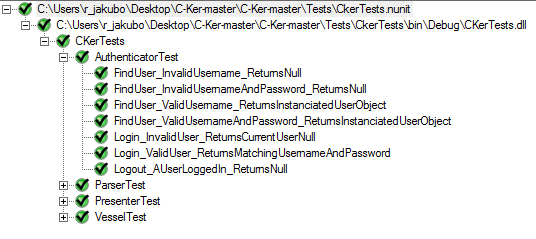
\includegraphics[scale=0.8]{Authenticator_class}
    \caption{Authenticator class}
    \label{fig:Authenticator class}
\end{figure}





\subsubsection{Requirements Testing}

This section contains a table (table~\ref{tab:Requirements Testing Part 1} \& ~\ref{tab:Requirements Testing Part 2}) that elaborates on the tests that we performed in order to validate the various use cases implemented in the final iteration of the C-Ker Vessel Monitoring System.

\clearpage

\begin{table}[ht]
\centering
   \begin{tabular}{|l|l|l|l|}
        \hline
        {\large Case} & {\large Input} & {\large Expected Result} & {\large Result}\\
        \hline\hline
        \multicolumn{4}{|l|}{1. Listing Vessels in a Table} \\
        \hline
        Default scenario file & Load & Vessels within range & OK\\
        "comp354\_vessel.vsf" & "comp354\_vessel.vsf" & are listed in the table, & \\
        is chosen &  into simulator &   and are added and &\\
         & & deleted as they move &\\
         & & in and out of range & \\
        \hline
        \multicolumn{4}{|l|}{2. Displaying Vessels on a Radar} \\
        \hline
       Default scenario file & Load & Vessels within range & OK\\
       "comp354\_vessel.vsf" & "comp354\_vessel.vsf" & are displayed on the &\\
       is chosen & into simulator & radar, and disappear &\\
        & & and appear as they & \\
        & & move in and out of & \\
        & & range &\\
        \hline
        \multicolumn{4}{|l|}{3. Filtering Vessels by Type} \\
        \hline
       Unfiltered table/radar  & Uncheck "Human"  & "Human" vessels are  & OK\\
       view contains vessel  & checkbox & no longer displayed in & \\
       type "Human" &  & table/radar view &\\
        \hline
        Unfiltered table/radar  & Uncheck "Human"  & No change in   & OK\\
       view does not contain  & checkbox & table/radar view &\\
       vessel type "Human" &  &  &\\
       \hline
        \multicolumn{4}{|l|}{4. Sorting Vessels by Attribute} \\
        \hline
       Unsorted/sorted table  & Click on "Vessel ID"  & Table sorts vessels by & OK\\
       contains vessels with   &  field once & descending order   &\\
       unique "Vessel ID" &  & according to "Vessel  &\\
        & & ID"&\\
        \hline
        Unsorted/sorted table & Click on "Vessel ID" & Table sorts vessels by & OK\\
        contains vessels with & field twice & ascending order   &\\
       unique "Vessel ID"&  & according to "Vessel &\\
        & & ID"&\\
       \hline
        \multicolumn{4}{|l|}{5. Loading Vessel Scenario Files} \\
        \hline
       Loading a scenario file & Load  & Error message "File has  & OK\\
       with bad values & "scenario\_badvalues.vsf" & invalid formatting." Is &\\
        & into simulator & displayed &\\
        \hline
        Loading an empty & Load & Error message "File has & OK\\
        scenario file & "scenario\_empty.vsf" & invalid formatting." Is &\\
         & into simulator & displayed&\\
         \hline
    \end{tabular}
\caption{Requirements Testing Part 1}
\label{tab:Requirements Testing Part 1}
\end{table}



\clearpage

\begin{table}[ht]
\centering
   \begin{tabular}{|l|l|l|l|}
        \hline
        {\large Case} & {\large Input} & {\large Expected Result} & {\large Result}\\
        \hline\hline
        \multicolumn{4}{|l|}{6. Simulating Vessel Movement} \\
        \hline
        A scenario file & Load & Vessel blips move & OK\\
        containing vessels with & "scenario\_20vessels.vsf"  & across the radar and & \\
        non-zero X and/or Y &  into simulator & corresponding vessel &\\
        velocities is chosen & & coordinates change in &\\
         & & the table over a regular&\\
         & & interval&\\
        \hline
        \multicolumn{4}{|l|}{7. Triggering Risk Alarms} \\
        \hline
        A scenario file & Load "scenario\_2.vsf" & The table entries for & OK\\
        containing vessels with & into simulator & the corresponding&\\
        trajectories that & & vessels turn&\\
        intersect/are close to & & red/yellow, and the&\\
        each other is chosen & & alarm animations are&\\
         & & displayed on the radar&\\
         \hline
        \multicolumn{4}{|l|}{8. Login Authentication} \\
        \hline
       A valid administrator & Enter "admin" in the first & The user avatar & OK\\
       username is entered in & field & changes from the & \\
       the login screen & & default image to the& \\
        & & administrator image &\\
        \hline
        A valid administrator & Enter "admin\_" in the & There is no change in & OK\\
        username is entered, & first field & the user avatar &\\
        but is followed by a & & &\\
        space (depicted by '\_') &  & &\\
        \hline
       An invalid & Enter "admin" in the first & Error message "Invalid & OK\\
       password/username or & field, and "derp" in the & credentials; please try &\\
       combination of the two & second & again." is displayed &\\
       is entered & & & \\
        \hline
        \multicolumn{4}{|l|}{9. Maximum of 100 Vessels in Simulation} \\
        \hline
       A scenario file & Load & All vessels in the & OK\\
       containing 100 vessels & "scenario\_100vessels.vsf" & scenario that are & \\
       is chosen & Into simulator & within the scenario’s &\\
       & & range are displayed in &\\
       & & the table/radar view  &\\
       \hline
        \multicolumn{4}{|l|}{10. Shortest TIMESTEP of 0.5 Seconds in Simulation} \\
        \hline
       A scenario file & Load & The table and radar & OK\\
       containing a TIMESTEP & "scenario\_10delay.vsf" & views update twice &\\
       of 0.5 is chosen & into simulator & every second &\\
       \hline
    \end{tabular}
\caption{Requirements Testing Part 2}
\label{tab:Requirements Testing Part 2}
\end{table}

\clearpage


















\subsubsection{Stress Testing}

In the original Requirement Document, it was required for the system to support up to 100 ships. As basic stress test, we conceived a simulation file with a thousand ships. Surprisingly enough, the C-Ker can run it without any difficulties. The Radar display is obviously very crowded and almost unreadable, but it still functions accordingly. For the purpose of this simulated stress test, we will also push other limits, such as range, speeds, refresh rate and simulation duration. We know for a matter of fact, after all the previously mentioned tests, that within reasonable conditions, the C-Ker VMS functions properly. First, we could stress test parameters individually. First, push the range of the radar from the current 5,000 meters cap, up to 50,000 meters, and run a standard 100 ship simulation until all ships have left the radar’s range. Then, we could push the limits of the boat speeds to close-to jet-speed speeds, thus testing the efficiency of the refresh rate, followed by an increase in the refresh rate, to add additional stress on the computing aspect of the system. And finally, we could test de duration efficiency of the system by designing a simulation with a duration time above 24 hours.\par
Ultimately, if all of the individual stress test mentioned above pass without resulting in a system crash or else, we could throw one, last, ultimate stress test at the C-Ker, which would implicate the joining of all previously, mentioned individual parameter stress tests. This ultimate challenge simulation could be based on 2,000 vessels and more, up to 10,000 vessels, all in a timed pattern to ensure the presence of at least 200 vessels at any given time within the radar range, which itself would be increased to above 10,000 meters. A given number of those vessels could be given excessively high speed rates while the radar refresh rate could be lowered in order to refresh more often. All of this, with a timing configuration to ensure the presence of the said 200 vessels at anytime for about one week of run-time (168 hours). This should prove to be the ultimate test for any VMS of the scale and scope of the C-Ker.











%%%%%%%%%%%%%%%%%%%%%%%%%%%%%%%%%%%%%%%%%%%%%%%%%%%%%%%%%%%%%%
%                      System Delivery                  
%%%%%%%%%%%%%%%%%%%%%%%%%%%%%%%%%%%%%%%%%%%%%%%%%%%%%%%%%%%%%%

\section{System Delivery}

\subsection{Installation Manual}
\vspace*{0.2in}
\leftline{\textsc{Step 1: Downloading the system.}}
\vspace*{0.2in}
First, head to \url{https://github.com/Darkneon/C-Ker} to reach our download page. There you will find C-Labs repository for the C-Ker VMS. On the bottom right of this page, you will find a button identified as “Download ZIP” (see figure~\ref{fig:Download ZIP}). Click it to start the download of your software.
\begin{figure}[h!]
    \centering
    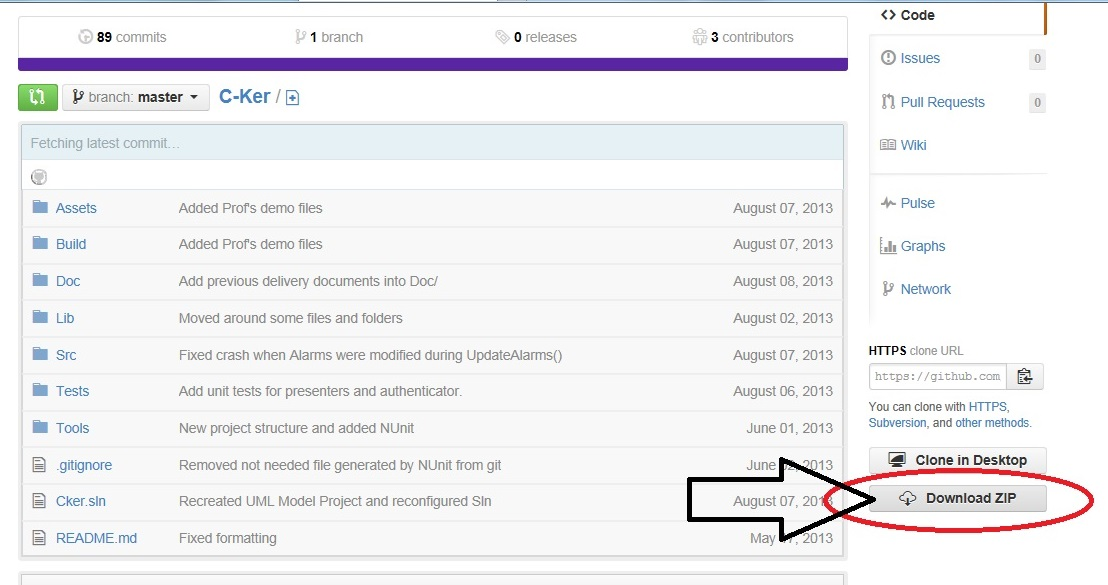
\includegraphics[scale=1]{insta1}
    \caption{Download ZIP}
    \label{fig:Download ZIP}
\end{figure}\par

Once you have located and clicked on the previously mentioned button, a box should prompt you to take action, by either Opening or Saving the ZIP file, or cancelling the operation. It is strongly recommended to Save the ZIP. More so, you should save it in a location of your choice by clicking on the smaller arrow next to the Save button on the prompt box (see figure~\ref{fig:Save}), which will expose a Scroll box from which you should select “Save as”. From Save as, select the location of your choice for the C-Ker master ZIP file. Depending on your browser and its version, the prompt box you see may be different than the one you currently see in the image below. If you are experimenting difficulties with the download prompt box of your web browser, you are strongly recommended to visit your browser’s manufacturer instruction manual.
\begin{figure}[h!]
    \centering
    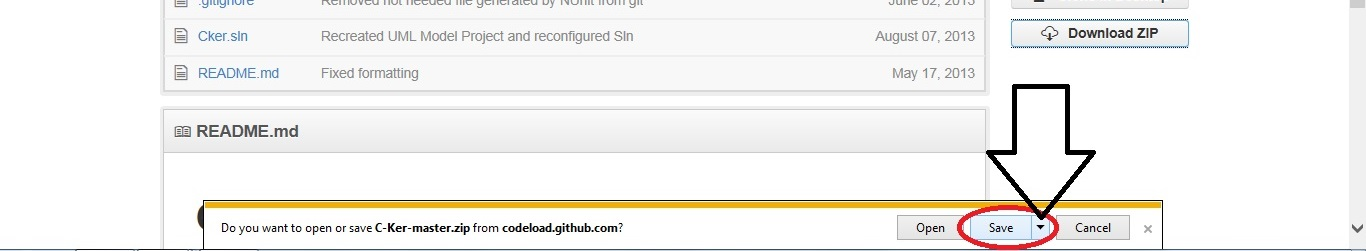
\includegraphics[scale=1]{insta2}
    \caption{Save}
    \label{fig:Save}
\end{figure}\par

Once you have saved the master ZIP file to the location of your choice, you may now proceed to the next step.\par


\vspace*{0.2in}
\leftline{\textsc{Step 2: Unzipping the Master File}}
\vspace*{0.2in}
Now that you have saved the master ZIP file at the location of your choice, locate it in its folder using Windows Explorer. If you cannot locate the ZIP file, repeat step 1 and try another location that could be easier for you to find. Once you have located the ZIP file (see figure~\ref{fig:Open ZIP file}), double left click it in order to open it.
\begin{figure}[h!]
    \centering
    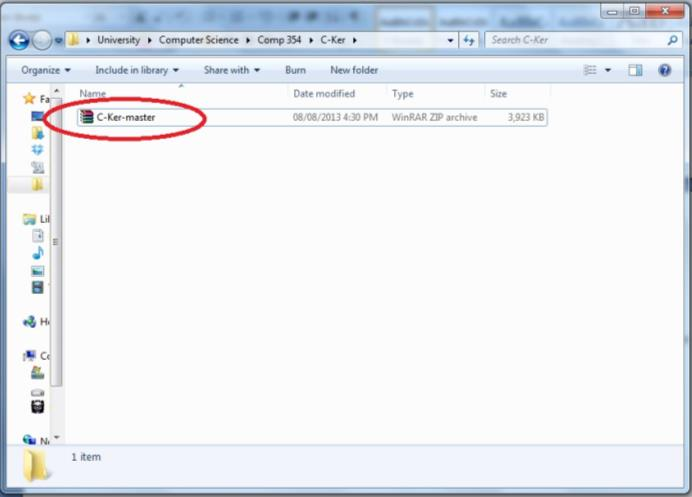
\includegraphics[scale=1]{insta3}
    \caption{Open ZIP file}
    \label{fig:Open ZIP file}
\end{figure}\par

Once you have double left clicked on the ZIP file, you should see the following screen opening (see figure~\ref{fig:ZIP file}), if not try again.
\begin{figure}[h!]
    \centering
    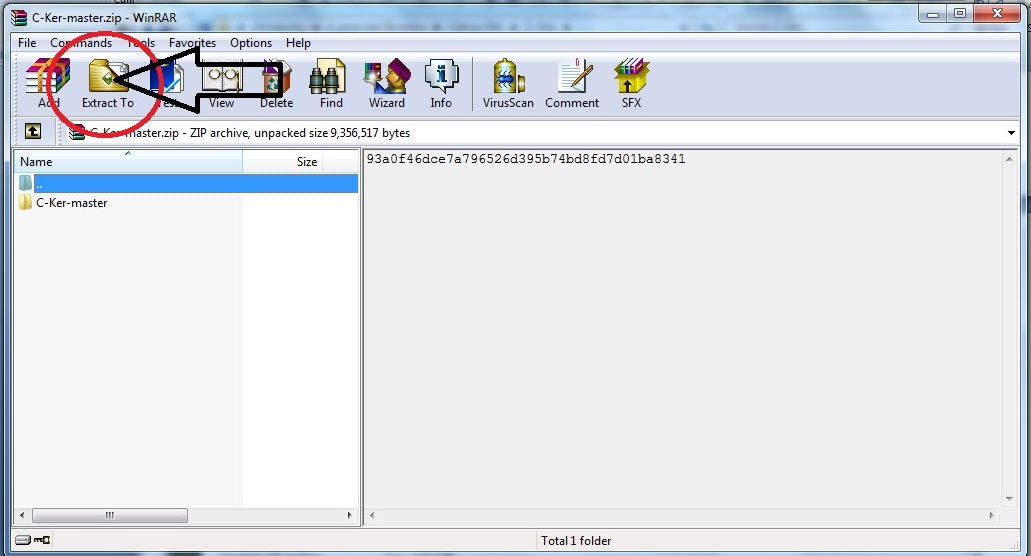
\includegraphics[scale=1]{insta4}
    \caption{ZIP file}
    \label{fig:ZIP file}
\end{figure}\par

Once you have the ZIP file opened (figure~\ref{fig:ZIP file}), left click once on the button identified “Extract to”. It will open a different window to ask you where you wish to extract the files (see figure~\ref{fig:Extract file}). If the new window does not open, click again.
\begin{figure}[h!]
    \centering
    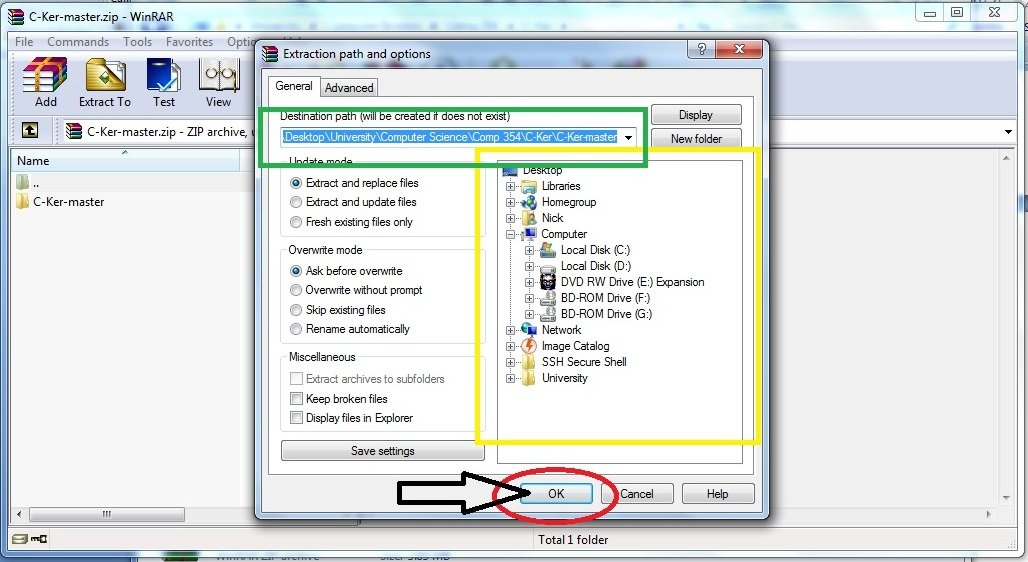
\includegraphics[scale=1]{insta5}
    \caption{Extract file}
    \label{fig:Extract file}
\end{figure}\par

Once the new window is opened, you will have the possibility to select the target location of your choice, either by typing the address (green box in figure~\ref{fig:Extract file}) or using the explorer display (yellow box in figure~\ref{fig:Extract file}). Once you are satisfied with your target location, click on the “OK” button (red circle in figure~\ref{fig:Extract file}). This will extract the ZIP file to the folder you selected, and create a new sub folder called “C-Ker-master” (see figure~\ref{fig:C-Ker-master}). 
\begin{figure}[h!]
    \centering
    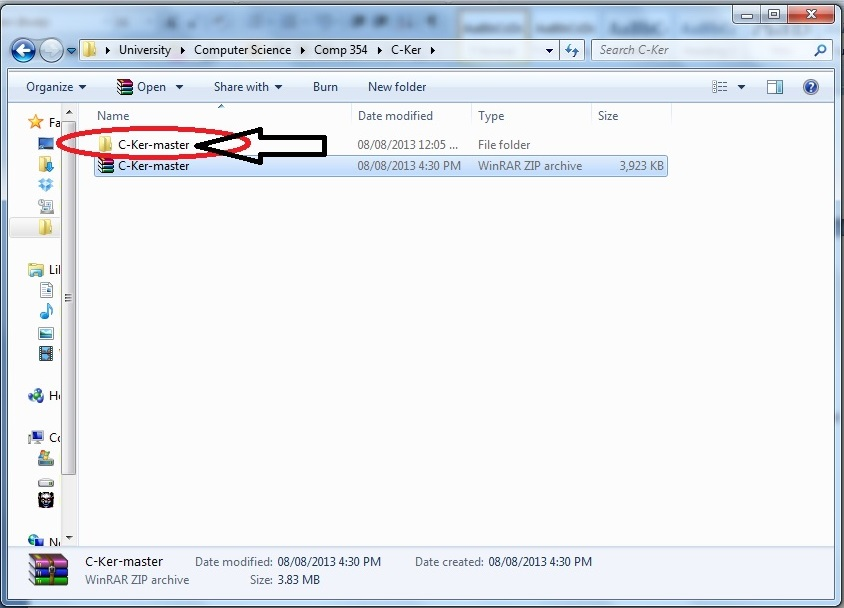
\includegraphics[scale=1]{insta6}
    \caption{C-Ker-master}
    \label{fig:C-Ker-master}
\end{figure}\par

\clearpage

If you can see the folder, then you have successfully unzipped the file and are ready to proceed to the next step.\par



\vspace*{0.2in}
\leftline{\textsc{Step 3: Running the VMS.}}
\vspace*{0.2in}
To reach the executable file of C-Ker, start by double clicking on the new folder created in step 2 in order to access its content. Once it is open, you should have the view as seen in figure~\ref{fig:Openned C-Ker-master folder}.
\begin{figure}[h!]
    \centering
    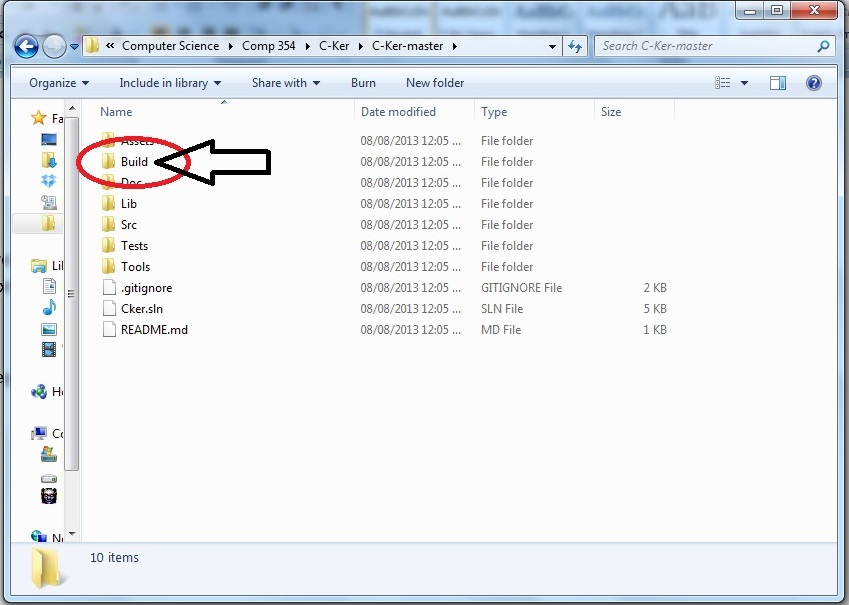
\includegraphics[scale=1]{insta7}
    \caption{Openned C-Ker-master folder}
    \label{fig:Openned C-Ker-master folder}
\end{figure}\par

Now that you have accessed the content of the C-Ker Master folder, locate the “Build” folder and double click it to open it.
\begin{figure}[h!]
    \centering
    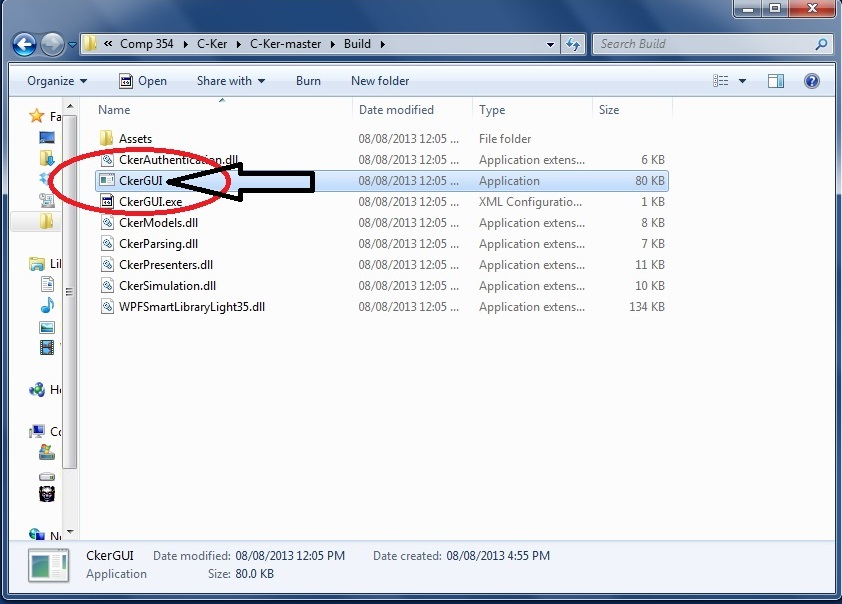
\includegraphics[scale=1]{insta8}
    \caption{CKerGUI}
    \label{fig:CKerGUI}
\end{figure}\par

Once this is done, locate the file named “CkerGUI” (pointed at by black arrow in figure~\ref{fig:CKerGUI}) and double click it to launch the C-Ker VMS.\\

{NOTE: Your computer may be running on a previous version of .NET Frameworks. If you receive an error message when trying to launch CkerGUI, head to the following hyperlink and follow the instructions to update your computers .NET Framework.}\\ 
\url{http://dotnetsocial.cloudapp.net/GetDotnet?o1=.NETFramework,Version=v4.5}\par
If everything works accordingly, you should see what is in figure~\ref{fig:CKer login screen} appears in the screen.
\begin{figure}[h!]
    \centering
    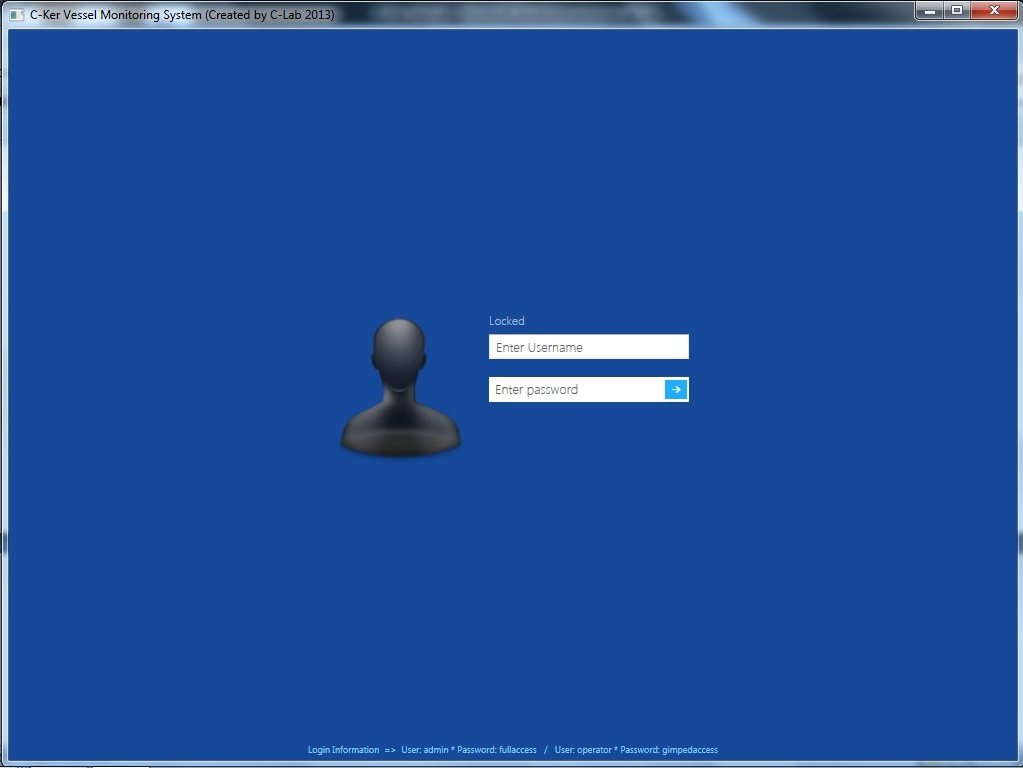
\includegraphics[scale=1]{insta9}
    \caption{CKer login screen}
    \label{fig:CKer login screen}
\end{figure}\par







\subsection{Users Manual}

In both of the following cases, the first, unmentioned, step is to launch the system. If you need instruction on how to launch C-Ker, refer to 1. Installation Manual – Step 3. 

\begin{enumerate} [(a)]
\vspace*{0.2in}
\item Operator Instructions\\
As C-Ker ‘Operator’ type user, enter “operator” as Username and “gimpedaccess” as password. Forgot your password and/or Username? They are on display at the bottom of the log in screen (see figure~\ref{fig:Logging In}).
\begin{figure}[h!]
    \centering
    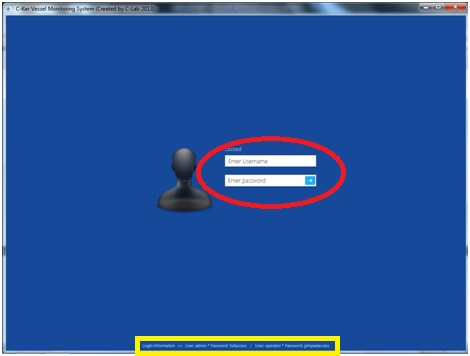
\includegraphics[scale=1]{manu1}
    \caption{Logging In}
    \label{fig:Logging In}
\end{figure}\par
Once you have completed your login, you should have access to the main page, which at this point should be blank. In order to load a simulation, click on the “New Simulation” button at the top left corner of the system (red square in figure~\ref{fig:New Simulation}), and a drop down box will appear with a list of preloaded simulations (yellow box in figure~\ref{fig:New Simulation}). If you wish to import and/or run a simulation from another, not preset, location, click on the “Browse” button (green square in figure~\ref{fig:New Simulation}), and a standard Windows Explorer file loader menu will open. Once you have found the simulation file of your choice, either in the preset menu or “Browse” section, simply double click on the file to open it and load the simulation onto the VMS. Once this is done, your simulation should be playing and C-Ker should be displaying something similar to the figure~\ref{fig:Operator View}. If you wish to load a new simulation simply repeat the step mentioned before and the new simulation will immediately replace the current one. To quit or change log in type, exit the system using the red “X” at the top right corner of the software, like any other software. For a full glossary of the icons displayed on the C-Ker, jump to section c) Glossary \& References.
\begin{figure}[h!]
    \centering
    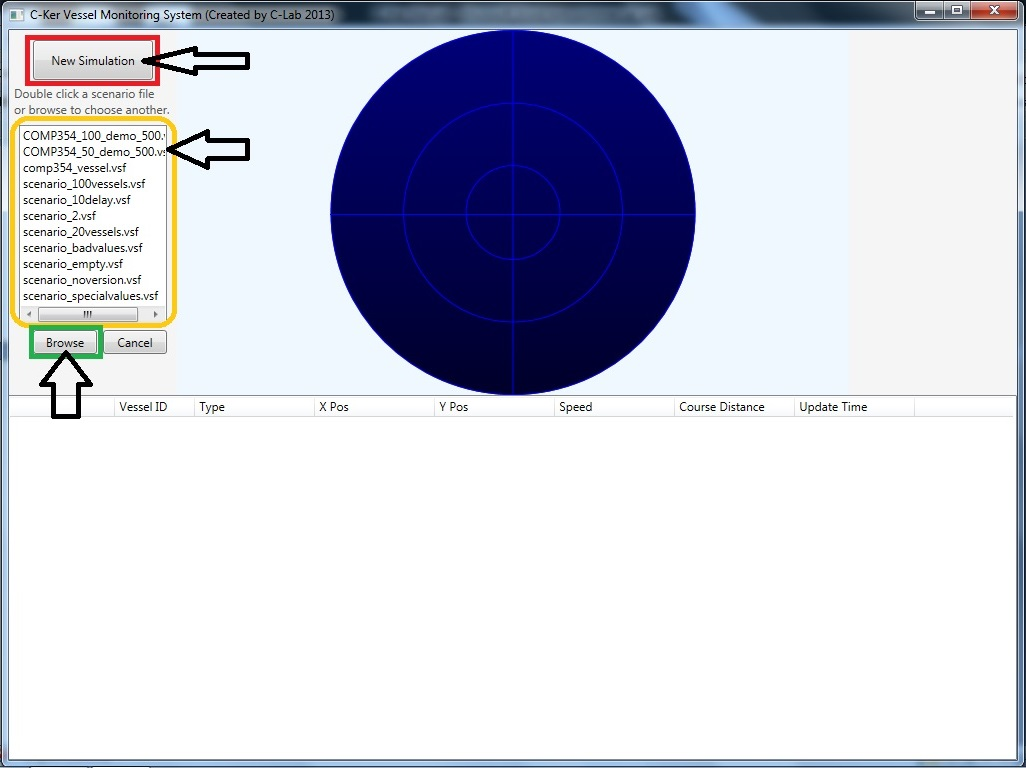
\includegraphics[scale=1]{manu2}
    \caption{New Simulation}
    \label{fig:New Simulation}
\end{figure}\par
\clearpage
\begin{figure}[h!]
    \centering
    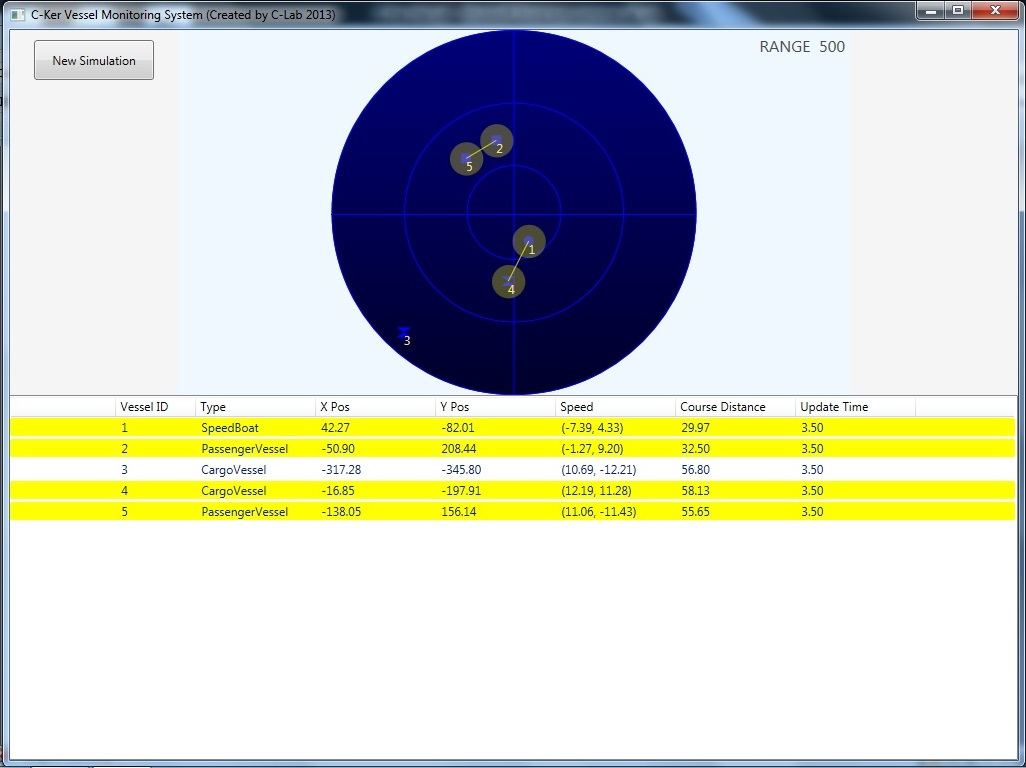
\includegraphics[scale=1]{manu3}
    \caption{Operator View}
    \label{fig:Operator View}
\end{figure}\par



\vspace*{0.2in}
\item Administrator Instructions\\
The log in instruction for Administrator access is the same as for an Operator access. Simply use the Username “admin” and password “fullaccess” to gain access to the C-Ker in Administrator mode. The loading of a simulation uses the same procedure as for the Operator access.  Once the selected simulation has loaded, you will gain access to two features unavailable in the Operator access: Sorting and Filtering vessels.
\clearpage
\begin{figure}[h!]
    \centering
    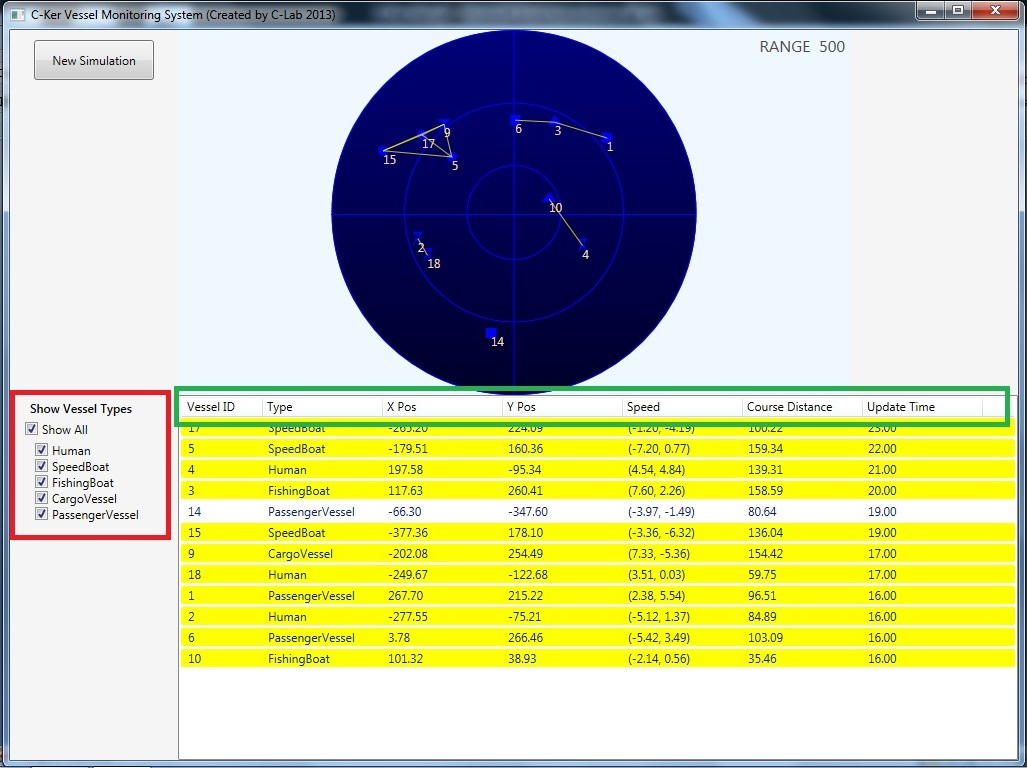
\includegraphics[scale=1]{manu4}
    \caption{Administrator View}
    \label{fig:Administrator View}
\end{figure}\par

Vessel Filtering:\\
In order to filter vessels, use the checkboxes at the left of the tab (red box in figure~\ref{fig:Administrator View}). If you wish to hide/show all vessels, click the checkbox names “Show All”. It will either hide or show all vessels both on the radar display and tab.  If you wish to either hide or show a specific type of vessel, check or uncheck its corresponding checkbox. \par

Vessel Sorting:\\
In order to sort vessels in the tab display, click on the parameter’s column by which you wish to sort the vessels (green box in figure~\ref{fig:Administrator View}). Depending on the current sorting method of the tab, click once on the parameter’s column of your choice will sort the vessels from smallest to largest parameter value, and twice will sort it from largest to lowest parameter value. Note that all 7 columns can be sorted.

\clearpage

\vspace*{0.2in}
\item Glossary \& References\\
\leftline{\textsc{Glossary}}
\begin{itemize}
\item Human (swimmer)\\
Represented by the hollow-X shape (figure~\ref{fig:Human (swimmer)})
\begin{figure}[h!]
    \centering
    
\includegraphics[scale=1]{leg1}
    \caption{Human (swimmer)}
    \label{fig:Human (swimmer)}
\end{figure}\par

\item Fishing Boat\\
Represented by the Triangle (figure~\ref{fig:Fishing Boat})
\begin{figure}[h!]
    \centering
    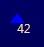
\includegraphics[scale=1]{leg2}
    \caption{Fishing Boat}
    \label{fig:Fishing Boat}
\end{figure}\par

\item Speed Boat\\
Represented by the Circle (figure~\ref{fig:Speed Boat})
\begin{figure}[h!]
    \centering
    
\includegraphics[scale=1]{leg3}
    \caption{Speed Boat}
    \label{fig:Speed Boat}
\end{figure}\par

\item Cargo Ship\\
Represented by Hourglass (figure~\ref{fig:Cargo Ship})
\begin{figure}[h!]
    \centering
    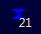
\includegraphics[scale=1]{leg4}
    \caption{Cargo Ship}
    \label{fig:Cargo Ship}
\end{figure}\par

\item Passenger Ship\\
Represented by the Square (figure~\ref{fig:Passenger Ship})
\begin{figure}[h!]
    \centering
    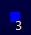
\includegraphics[scale=1]{leg5}
    \caption{Passenger Ship}
    \label{fig:Passenger Ship}
\end{figure}\par
\end{itemize}




\leftline{\textsc{Reference}}
The following reference section will provide additional information and clarification about items not shown prior.\par
\begin{figure}[h!]
    \centering
    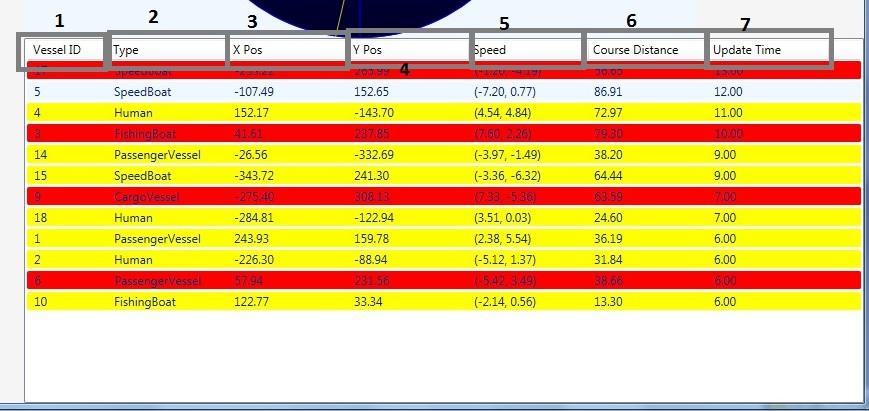
\includegraphics[scale=1]{ref1}
    \caption{Tab Display}
    \label{fig:Tab Display}
\end{figure}\par

Tab Display (figure~\ref{fig:Tab Display}):
\begin{enumerate}[(1)]
\item Vessel ID:\\
The number ID assigned to the ship
\item Type:\\
Type of vessel
\item X Pos:\\
Location on the East-West ‘X’ axis
\item Y Pos:\\
Location on the North-South ‘Y’ axis
\item Speed:\\
Velocity at which the vessel is currently traveling
\item Course Distance:\\
Distance from Radar ‘Origin’ (0, 0)
\item Update Time:\\
Total time since vessel has appeared on the VMS
\end{enumerate}

\vspace*{0.2in}

\begin{figure}[h!]
    \centering
    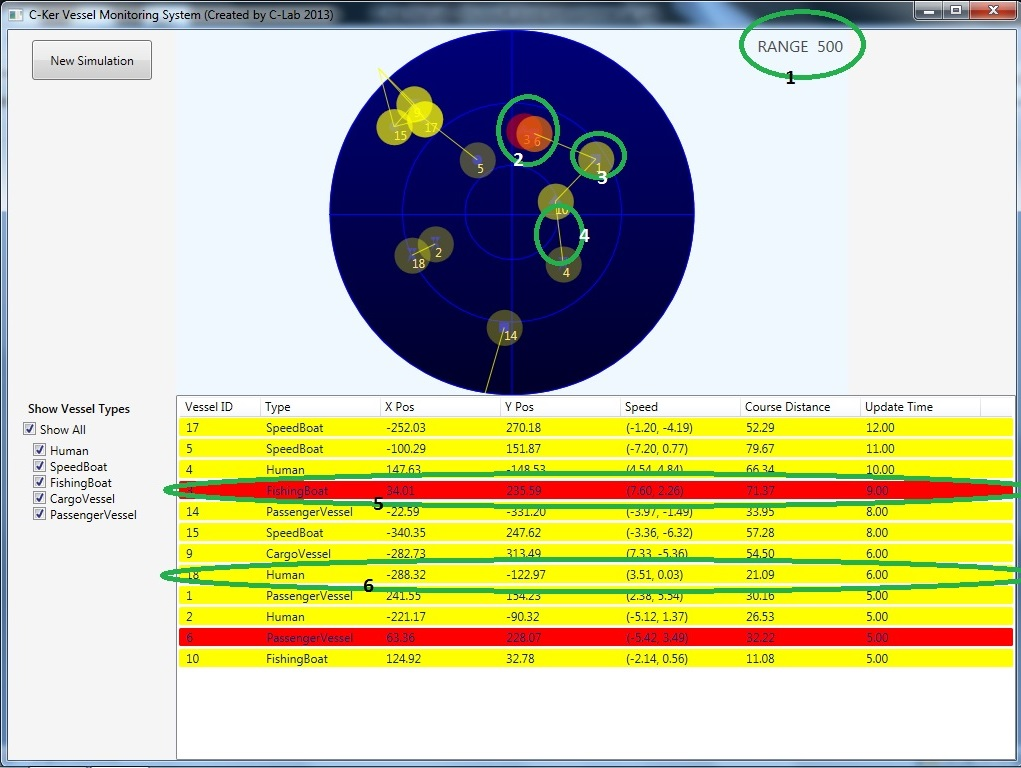
\includegraphics[scale=1]{ref2}
    \caption{Radar Display}
    \label{fig:Radar Display}
\end{figure}\par

Radar display (figure~\ref{fig:Radar Display}):
\begin{enumerate}[(1)]
\item Range\\
The Range at which the radar is set. Equivalent to the radius of the circle of the radar
\clearpage
\item Glowing Red Circle\\
Indicates the ship at the center of the circle is in high danger of collision, and is within 50 meters of another ship
\item Glowing Yellow Circle\\
Indicated the ship at the center of the circle is potentially in danger of collision, and is between 50 and 200 meters away from another ship
\item Yellow Line\\
Indicates the relationship between two ships in mutual Yellow Alert
\item Red Tab Line\\
Indicates, within the tab display, that a ship is in high danger of collision, same as 2- Glowing Red Circle
\item Yellow Tab Line\\
Indicated, within the tab display, that a ship is potentially in danger of collision, same as 3- Glowing Yellow Circle



\end{enumerate}






\end{enumerate}


%%%%%%%%%%%%%%%%%%%%%%%%%%%%%%%%%%%%%%%%%%%%%%%%%%%%%%%%%%%%%%
%                    Final cost estimate                    
%%%%%%%%%%%%%%%%%%%%%%%%%%%%%%%%%%%%%%%%%%%%%%%%%%%%%%%%%%%%%%

\section{Final cost estimate}


With the delivery of the completed product comes the time to assess the cost associated with the development of the said product.  In order to pinpoint as accurately as possible the total cost of the development of the C-Ker VMS, we will evaluate the following points.

\clearpage
\subsection{Technical Resources}
    Since Delivery 1, our technical resource estimation and consumption has not changed, except for maybe a language library.  We have not changed anything, compiler software, repository or language. Since everything we use was free, either a free service or software licensed via ENCS, we cannot account for any costs. 
\subsection{Time/Human Resources Cost}
	The entire cost evaluation and calculation of the project resides on the time and human resources consumed for the realisation of the C-Ker.  As most hours worked on an item or another were registered by the members of C-Labs into a time log, we are capable of safely estimating the exact cost in hours of the development process. \par
	Generally speaking, the documentation task for the delivery of this project used roughly 50\% of the time put into the project by the members of C-Labs. According to the time logs of each member, about 320 hours of man-time went into this project, spread across our 5 members. We consider the time logs only as indicators and not accurate counter, as the proper use of the time log was not implemented early in the project, but rather just in time for delivery 3. The programmers logged a few less hours than the documentation/administration team, most likely because they did not consider the meeting times into their logs. It is our believe that everyone on C-labs has worked more hours than stipulated in time logs, but since this is only a cost estimate and not an accurate cost calculation, we will work with those numbers.\par
	Ash and Brian had similar time consumption percentage and a similar total of hours, both been around 40-50 hours spent, with about 50\% of their time dedicated to coding/programming or similar functions, and 50\% of their time documenting. On the other hand, Robert, with his technical leader responsibilities, spent about 60 hours split in three, roughly even, parts: development, deployment and designing, the last which includes documentation for the designs.\par
	On the contrary, Nick and Caro’s time were above that of Robert’s 60 hours, and were mostly dedicated to documenting, note taking and team coordination. They did spent some time testing and running the program in order to help the programming team with the testing phase of the delivery.
\subsection{Incalculable Costs}
	Considering this is a non-complete Cost Evaluation based on a school project, many costs items had to be left behind unconsidered and uncalculated. For a starter, even if the Human Resources consumption was calculated in hours, wages are not considered in our evaluation. Also, since we used the optimal programming language that suited our main programmers best, we did not have to waste any resources on training on new technical items. Furthermore, everything regarding overhead expenditures, such as rent, electricity, and insurance, is ignored. For the hardware and software costs, we are also negating those as we did not purchase anything for this project, therefore, we will also negate the amortisation on the cost. Also, we were not able to reuse code from previous project, as none of us had worked on a VMS before. Exception made for a few items for the log in system, but not enough to be noticeable. In the same line of thought, we will not be able to reuse most of the code from the C-Ker since it is too specialized, and thus cannot be calculated as recovered cost.
    
    \clearpage
\subsection{Risk Induced Costs}
	This project was blessed with a minimal amount of risk factor actually happening.  Most of the duration of the project went without any major issues but one noticeable incident. One team member had health issues within her family, and had to miss a few team meetings and could not provide the same amount of work as plan. Thankfully, she managed to get her section done in time as the rest of the team picked up the slack, noting the Meeting Minutes and so on, which resulted in very little impact on the final result. Also, it is fair to say that every team member had his off moment at a time or another, where emails were not returned promptly, or the level of implication was not to the expected level. In the end, not only did it had no effect on the final result, but the team was proficient enough that no team member ever needed to be brought back in line or asked to raise the level of production.


%%%%%%%%%%%%%%%%%%%%


\end{document}